\section{应用：带噪递推的稳定与收敛}
\label{sec:dtsp-stochastic-approximation}

最后一节把鞅累计、长期平均与确定性稳定性合起来，用于分析一类随机递推：每一步只能拿到带噪声的信息，却希望参数最终停在某个方程的根上。随机梯度下降是最常见的实例，但这里研究的对象是递推路径本身及其平均漂移，不是优化算法的目录；算法的设计与有限预算下的进展由优化部分讨论（第~\ref{chap:opt-stochastic-block}章），这里回答的是：随机轨迹为什么会稳定、在什么条件下收敛。

\subsection{随机求根与递推误差}
\label{sec:dtsp-root-finding}

\paragraph{只能观测带噪响应时的求根}
设想要找一个剂量$\theta$，使某种反应的平均强度恰好等于目标值。每做一次试验只能看到一个带噪声的读数，平均反应函数本身未知。形式上，有一个平均漂移$\overline h(\theta)=\mathbb E[H(\theta,Y)]$，我们只能在选定的$\theta$处取得$H(\theta,Y)$的一个随机实现，目标是找到$\overline h(\theta^\star)=0$的根。\term{随机逼近}（stochastic approximation）的基本递推是
\begin{equation}
  \bm\theta^{(n+1)}=\bm\theta^{(n)}+\alpha_n\bm H(\bm\theta^{(n)},Y_{n+1}),
  \label{eq:dtsp-robbins-monro}
\end{equation}
其中$\alpha_n>0$是步长\scite{math-robbins1951stochastic}。迭代编号用带括号的上标，与物理时间下标区分。按照Doob分解的思路，把每一步拆成三部分：
\begin{equation}
  \bm H(\bm\theta^{(n)},Y_{n+1})=\overline{\bm h}(\bm\theta^{(n)})+\bm\xi_{n+1}+\bm r_{n+1},
  \label{eq:dtsp-sa-decomposition}
\end{equation}
其中$\overline{\bm h}(\bm\theta^{(n)})$是平均漂移，$\bm\xi_{n+1}$满足$\mathbb E[\bm\xi_{n+1}\mid\mathcal F_n]=\bm 0$，是鞅差噪声，$\bm r_{n+1}$收集近似、截断或观测尚未平衡带来的偏差。分析的路线也随之确定：漂移部分用确定性稳定性处理，噪声部分用第~\ref{sec:dtsp-deviation}节的鞅工具处理，偏差部分须单独证明可以忽略。

三个例子说明这个框架有多宽。估计均值：$H(\theta,Y)=Y-\theta$，根为$\mu=\mathbb EY$；取$\alpha_n=1/(n+1)$，由归纳得$\theta^{(n)}=\frac1n\sum_{k\leq n}Y_k$，样本平均就是一种随机逼近。估计分位数：$H(\theta,Y)=q-\mathbb I\{Y\leq\theta\}$，平均漂移为$q-F(\theta)$，根是$q$分位数；每步只需一次比较，噪声有界。随机梯度：$\bm H(\bm\theta,Y)=-\nabla_{\bm\theta}\ell(\bm\theta,Y)$，在可交换微分与期望时平均漂移为$-\nabla L(\bm\theta)$，根是平均损失的驻点。

\paragraph{方程的根、计算误差与统计误差}
随机逼近收敛到的是所选方程$\overline h=0$的根。这个根是否就是我们真正关心的量，是建模问题，不是收敛问题：只有当模型正确、目标与方程的关系成立时，根才代表所需的参数。若递推运行在一组固定的数据上（例如对有限样本的平均损失做随机梯度），总误差可以分成两部分：迭代与该数据集上的根之间的计算误差，以及该根与总体目标之间的统计误差。本节只讨论前者。若数据在线到达、每步用一个新样本，样本数与迭代次数一起增长，计算误差与统计误差交织在一起，需要联合论证。统计误差的大小、效率与置信区间可参考\BookChapterRef{chap:statistical-inference}{卷四“统计推断”章}。

\subsection{步长、噪声与路径稳定}
\label{sec:dtsp-stepsizes}

\paragraph{两个步长条件的作用}
经典的递减步长条件是
\begin{equation}
  \sum_{n\geq0}\alpha_n=\infty,\qquad\sum_{n\geq0}\alpha_n^2<\infty.
  \label{eq:dtsp-robbins-monro-steps}
\end{equation}
两条分别对付两个敌人。第一条保证累计移动能力无限：若$\sum\alpha_n<\infty$，即使没有噪声，迭代也可能在到达根之前就“走不动了”，例如$\theta^{(n+1)}=\theta^{(n)}-\alpha_n\theta^{(n)}$的解是$\theta^{(0)}\prod(1-\alpha_k)$，在$\sum\alpha_k<\infty$时不趋于零。第二条控制累计噪声：噪声以$\alpha_n\bm\xi_{n+1}$的形式进入，若条件方差有统一上界$\sigma^2$，定理~\ref{thm:dtsp-weighted-martingale-sum}说明$\sum_n\alpha_n\bm\xi_{n+1}$几乎必然收敛，噪声的总影响有限。$\alpha_n=c/(n+n_0)^\gamma$在$c,n_0>0$、$\frac12<\gamma\leq1$时满足两条。仅有每一步方差有限还不够，因为方差可能随时间无界增长。

\paragraph{标量线性递推的收敛}
先在最简单的情形中把这两个条件与第~\ref{sec:dtsp-weighted-noise}节的几乎超鞅定理接起来。

\begin{theorem}[标量线性随机逼近]
  \label{thm:dtsp-scalar-sa}
  设$\theta^{(n+1)}=\theta^{(n)}+\alpha_n(b-a\theta^{(n)}+\xi_{n+1})$，其中$a>0$，$\mathbb E(\theta^{(0)})^2<\infty$，$\mathbb E[\xi_{n+1}\mid\mathcal F_n]=0$，$\mathbb E[\xi_{n+1}^2\mid\mathcal F_n]\leq\sigma^2$，确定步长满足式~\eqref{eq:dtsp-robbins-monro-steps}。则$\theta^{(n)}\to b/a$几乎必然。
\end{theorem}

\begin{proof}
记误差$e_n=\theta^{(n)}-b/a$，则$e_{n+1}=(1-a\alpha_n)e_n+\alpha_n\xi_{n+1}$，各$e_n$平方可积。$\alpha_n\to0$，舍去有限个初始步，可设$a\alpha_n\leq1$。展开平方并取条件期望，交叉项因$\xi$条件均值为零而消失：
\[
  \mathbb E[e_{n+1}^2\mid\mathcal F_n]=(1-a\alpha_n)^2e_n^2+\alpha_n^2\mathbb E[\xi_{n+1}^2\mid\mathcal F_n]\leq e_n^2-a\alpha_ne_n^2+\alpha_n^2\sigma^2.
\]
这正是式~\eqref{eq:dtsp-almost-supermartingale}，取$Z_n=e_n^2$、$\beta_n=0$、$b_n=\alpha_n^2\sigma^2$、$A_n=a\alpha_ne_n^2$。定理~\ref{thm:dtsp-almost-supermartingale}给出$e_n^2$几乎必然收敛到某个$L$，且$\sum_n\alpha_ne_n^2<\infty$。若某条路径上$L>0$，最终$e_n^2\geq L/2$，便有$\sum_n\alpha_ne_n^2\geq\frac L2\sum_n\alpha_n=\infty$，矛盾。所以$L=0$。
\end{proof}

证明清楚地显示了两个步长条件各自的位置：平方可和使$b_n$可求和，和发散使“累计下降有限”迫使误差趋零。取$a=1$、$b=\mu$就得到均值递推的收敛。

\paragraph{非线性情形：Lyapunov函数}
同一论证可以推广到非线性漂移，只要能找到一个沿平均漂移下降的“能量”。

\begin{theorem}[强单调漂移下的几乎必然收敛]
  \label{thm:dtsp-sa-lyapunov}
  设式~\eqref{eq:dtsp-robbins-monro}中$\bm r_{n+1}=\bm 0$，并存在$\bm\theta^\star$与常数$c>0$、$K<\infty$，使对所有$\bm\theta$，
  \[
    \begin{aligned}
      &\langle\bm\theta-\bm\theta^\star,\overline{\bm h}(\bm\theta)\rangle\leq-c\lVert\bm\theta-\bm\theta^\star\rVert_2^2,\\
      &\mathbb E\bigl[\lVert\bm H(\bm\theta^{(n)},Y_{n+1})\rVert_2^2\bigm|\mathcal F_n\bigr]\leq K\bigl(1+\lVert\bm\theta^{(n)}-\bm\theta^\star\rVert_2^2\bigr).
    \end{aligned}
  \]
  若$\mathbb E\lVert\bm\theta^{(0)}\rVert_2^2<\infty$且确定步长满足式~\eqref{eq:dtsp-robbins-monro-steps}，则$\bm\theta^{(n)}\to\bm\theta^\star$几乎必然。
\end{theorem}

\begin{proof}
令$Z_n=\lVert\bm\theta^{(n)}-\bm\theta^\star\rVert_2^2$。展开$\bm\theta^{(n+1)}-\bm\theta^\star=(\bm\theta^{(n)}-\bm\theta^\star)+\alpha_n\bm H$的平方并取条件期望，一次项中$\mathbb E[\bm H\mid\mathcal F_n]=\overline{\bm h}(\bm\theta^{(n)})$，于是
\[
  \mathbb E[Z_{n+1}\mid\mathcal F_n]\leq Z_n-2c\alpha_nZ_n+\alpha_n^2K(1+Z_n)=(1+K\alpha_n^2)Z_n+K\alpha_n^2-2c\alpha_nZ_n.
\]
由归纳，每个$Z_n$可积。定理~\ref{thm:dtsp-almost-supermartingale}（$\beta_n=b_n=K\alpha_n^2$，$A_n=2c\alpha_nZ_n$）给出$Z_n$收敛且$\sum\alpha_nZ_n<\infty$，再用$\sum\alpha_n=\infty$同前得极限为零。
\end{proof}

对随机梯度，第一条件就是平均损失的强凸性（$\overline{\bm h}=-\nabla L$，$L$为$c$强凸），第二条件允许梯度噪声的二阶矩随距离平方增长。两条都不能简单删去：没有漂移条件，迭代可能停在其他驻点或在多个吸引集之间徘徊；没有增长条件，噪声可能把迭代推到更远处，使有界性本身失去保证。一般非线性递推往往先要单独证明迭代几乎必然有界，再研究它被吸引到哪里，这正是下一小节的平均ODE方法。

\paragraph{固定步长与递减步长}
递减步长追求收敛；固定步长$\alpha_n\equiv\alpha$则保留对新观测的持续响应，代价是迭代不再收敛到一点，而在根附近持续波动。对均值递推，若观测独立同分布、方差为$\sigma^2$，误差满足$e_{n+1}=(1-\alpha)e_n+\alpha(Y_{n+1}-\mu)$，于是
\[
  \mathbb Ee_n=(1-\alpha)^ne_0,\qquad
  \operatorname{Var}(e_n)\to\frac{\alpha\sigma^2}{2-\alpha}.
\]
初始偏差几何地消失，留下与步长成正比的稳态方差。图~\ref{fig:dtsp-robbins-monro}比较三种步长：$\alpha_n=1/(n+1)$（样本平均）的均方误差为$1/n$；$\alpha_n=(n+1)^{-0.6}$下降得较慢；$\alpha=0.2$的均方误差很快停在$0.2/1.8=1/9$。更一般地，标量线性递推在$|1-a\alpha|<1$时，若噪声独立同分布、方差$v>0$，稳态方差为$\alpha^2v/(1-(1-a\alpha)^2)$。仅有条件方差的上界只能推出稳态误差的上界；要断言波动确实为正，还需要噪声非退化。

\begin{figure}[htbp]
  \centering
  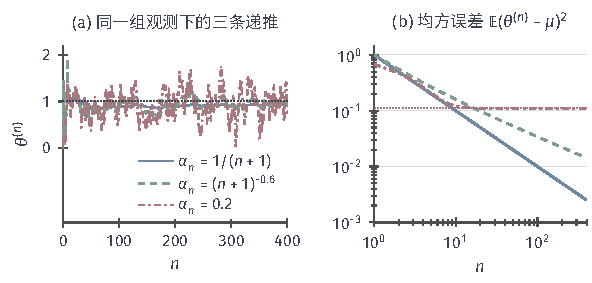
\includegraphics[width=100mm]{figures/03-optimization-evolution-and-signals/02-processes-and-trajectory-evolution/tikz/dtsp-robbins-monro/figure.pdf}
  \caption{均值估计的Robbins--Monro递推。观测独立服从$\mathcal N(1,1)$，$\theta^{(0)}=0$。(a)同一组模拟观测下三种步长的迭代路径；(b)由递推$m_{n+1}=(1-\alpha_n)^2m_n+\alpha_n^2$精确算出的均方误差（双对数坐标），点线为固定步长$0.2$的极限$1/9$。}
  \label{fig:dtsp-robbins-monro}
\end{figure}

\subsection{平均ODE与Markov噪声}
\label{sec:dtsp-ode-markov}

\paragraph{算法时钟与插值轨迹}
步长趋于零时，递推~\eqref{eq:dtsp-robbins-monro}的每一步都是对平均漂移的一个小Euler步，加上一点噪声。若用累计步长作为“时钟”，
\[
  \tau_0=0,\qquad\tau_n=\sum_{k<n}\alpha_k,
\]
并把点$(\tau_n,\bm\theta^{(n)})$用折线连起来，得到插值轨迹$\widehat{\bm\theta}(\tau)$，就可以把它与\term{平均ODE}（mean ODE）
\begin{equation}
  \dot{\bm\theta}(\tau)=\overline{\bm h}(\bm\theta(\tau))
  \label{eq:dtsp-mean-ode}
\end{equation}
的解比较。图~\ref{fig:dtsp-mean-ode-tracking}是一个二维线性例子：平均漂移$\overline{\bm h}(\bm\theta)=-\bm A\bm\theta$，$\bm A=\left(\begin{smallmatrix}0.5&-1\\1&0.5\end{smallmatrix}\right)$，平均ODE的解以$e^{-\tau/2}$的速度旋转着收缩。按迭代编号看，路径前段大步跳跃、后段挤成一团；按算法时间看，(b)中迭代的第一坐标紧紧跟着ODE解振荡衰减。

\begin{figure}[htbp]
  \centering
  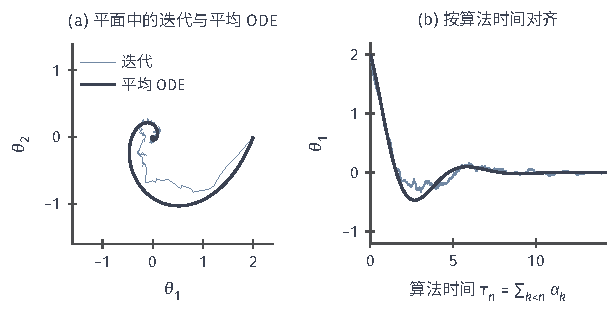
\includegraphics[width=104mm]{figures/03-optimization-evolution-and-signals/02-processes-and-trajectory-evolution/tikz/dtsp-mean-ode-tracking/figure.pdf}
  \caption{线性随机逼近与平均ODE。递推为$\bm\theta^{(n+1)}=\bm\theta^{(n)}+\alpha_n(-\bm A\bm\theta^{(n)}+\bm\xi_{n+1})$，$\bm A=\left(\begin{smallmatrix}0.5&-1\\1&0.5\end{smallmatrix}\right)$，$\bm\xi_n$独立服从$\mathcal N(\bm 0,0.64\bm I)$，$\alpha_n=0.6/(n+5)^{0.75}$，$\bm\theta^{(0)}=(2,0)$，共$3000$步（固定随机种子）。黑线为平均ODE的解$2e^{-\tau/2}(\cos\tau,-\sin\tau)$。(a)平面中的路径；(b)第一坐标对算法时间$\tau_n$。}
  \label{fig:dtsp-mean-ode-tracking}
\end{figure}

\term{ODE方法}（ODE method）把这一观察变成定理。它不要求每个随机增量都接近平均增量，只要求在任意长度固定的算法时间窗内，累计噪声和偏差最终可以忽略。一组常用的充分条件是：$\alpha_n\to0$且$\sum\alpha_n=\infty$；$\overline{\bm h}$局部Lipschitz；迭代几乎必然有界；对每个$T>0$，
\[
  \sup_{k\geq n,\ \tau_k-\tau_n\leq T}\Bigl\lVert\sum_{j=n}^{k-1}\alpha_j(\bm\xi_{j+1}+\bm r_{j+1})\Bigr\rVert_2\longrightarrow0\qquad\text{几乎必然}.
\]
鞅差部分的这一条件由定理~\ref{thm:dtsp-weighted-martingale-sum}保证：加权和几乎必然收敛，所以它的尾部在任何窗口上都一致趋于零。在这些条件下，插值轨迹在每个有限窗口上满足平均ODE的积分方程，只差一个一致趋零的残差；Grönwall不等式（见第~\ref{chap:ordinary-differential-equations}章）把残差转化为与ODE解的一致接近。这一步只连接了有限窗口内的轨迹；若平均ODE还有全局渐近稳定的平衡点$\bm\theta^\star$，并且它对迭代所在的紧集一致吸引，才能推出$\bm\theta^{(n)}\to\bm\theta^\star$\scite{math-borkar2008stochastic}。平均ODE若有多个吸引集，迭代可能落入其中任何一个；平均稳定也不意味着全局最优。

\paragraph{线性平均漂移的稳定条件}
对线性漂移$\overline{\bm h}(\bm\theta)=\bm b-\bm A\bm\theta$，平均ODE的误差满足$\dot{\bm e}=-\bm A\bm e$。由线性ODE的谱判据，$\bm A$的全部特征值实部为正时误差指数衰减。若对称部分$(\bm A+\bm A^{\top})/2$正定，欧氏能量$\frac12\lVert\bm e\rVert_2^2$本身就严格下降，因为反对称部分的二次型为零；图~\ref{fig:dtsp-mean-ode-tracking}的$\bm A$对称部分是$0.5\bm I$，属于这种情形。这一条件充分而不必要：$\bm A=\left(\begin{smallmatrix}1&10\\0&1\end{smallmatrix}\right)$的特征值都是$1$，对称部分却不定，欧氏误差可能先增大，换用由Lyapunov方程$\bm A^{\top}\bm P+\bm P\bm A=\bm Q$给出的二次型$\bm e^{\top}\bm P\bm e$才严格下降。

\paragraph{Markov观测与Poisson方程}
许多递推中，观测不是独立抽取的，而是来自一条Markov链：$\theta^{(n+1)}=\theta^{(n)}+\alpha_nH(\theta^{(n)},X_n)$，$X_n$以核$P$转移、不变分布为$\pi$。此时平均漂移是$\overline h(\theta)=\int H(\theta,x)\,\pi(\mathrm dx)$，但$H(\theta,X_n)-\overline h(\theta)$给定过去的条件均值一般不为零，它不是鞅差，第~\ref{sec:dtsp-weighted-noise}节的定理不能直接用。解决办法是第~\ref{sec:dtsp-ergodic-averages}节用过的Poisson方程：对固定的$\theta$求$g_\theta$，使
\[
  g_\theta-Pg_\theta=H(\theta,\cdot)-\overline h(\theta).
\]
代入后，相关误差被拆成一个鞅差和一个望远镜项：
\[
  H(\theta,X_n)-\overline h(\theta)=\underbrace{g_\theta(X_{n+1})-Pg_\theta(X_n)}_{\text{鞅差}}+\underbrace{g_\theta(X_n)-g_\theta(X_{n+1})}_{\text{相邻项相消}}.
\]
这里的Poisson方程是链的转移算子上的方程，与第~\ref{chap:partial-differential-equations}章空间区域上的Poisson边值问题名称相同，对象不同。

\begin{lemma}[有限链上的加权Poisson分解]
  \label{lem:dtsp-finite-poisson-sum}
  设$P$是有限状态上不可约、非周期的转移矩阵，迭代$\theta^{(n+1)}=\theta^{(n)}+\alpha_nH(\theta^{(n)},X_n)$始终位于紧集$K$，$H$在$K\times E$上有界且关于$\theta$一致Lipschitz，正步长单调递减且满足式~\eqref{eq:dtsp-robbins-monro-steps}。则$\sum_n\alpha_n[H(\theta^{(n)},X_n)-\overline h(\theta^{(n)})]$几乎必然收敛，从而它在任意有限算法时间窗上的尾和趋于零。
\end{lemma}

\begin{proof}
记$c_\theta=H(\theta,\cdot)-\overline h(\theta)$，$\pi(c_\theta)=0$。由定理~\ref{thm:dtsp-finite-convergence}，$g_\theta=\sum_{j\geq0}P^jc_\theta$一致绝对收敛，满足Poisson方程，并且存在常数$G,L_g$使$|g_\theta|\leq G$、$|g_\theta-g_{\theta'}|\leq L_g|\theta-\theta'|$（对$c_\theta-c_{\theta'}$用同样的几何界）。于是
\[
  \begin{aligned}
    \sum_{n\leq N}\alpha_nc_{\theta^{(n)}}(X_n)&=\sum_{n\leq N}\alpha_n\bigl[g_{\theta^{(n)}}(X_{n+1})-Pg_{\theta^{(n)}}(X_n)\bigr]\\
    &\quad+\sum_{n\leq N}\alpha_n\bigl[g_{\theta^{(n)}}(X_n)-g_{\theta^{(n)}}(X_{n+1})\bigr].
  \end{aligned}
\]
第一项是条件方差不超过$4G^2\alpha_n^2$的鞅差和，由定理~\ref{thm:dtsp-weighted-martingale-sum}收敛。第二项作分部求和，除去两个端点项外，中间各项为$\alpha_ng_{\theta^{(n)}}(X_n)-\alpha_{n-1}g_{\theta^{(n-1)}}(X_n)$，绝对值至多$G(\alpha_{n-1}-\alpha_n)+\alpha_{n-1}L_g|\theta^{(n)}-\theta^{(n-1)}|$；而$|\theta^{(n)}-\theta^{(n-1)}|\leq C\alpha_{n-1}$。前一部分由单调性望远镜求和，后一部分被$\sum\alpha_n^2$控制，端点项因$\alpha_n\to0$而消失。
\end{proof}

回到两状态链，取$H(\theta,x)=\mathbb I\{x=2\}-\theta$，递推估计长期拥堵比例$1/3$。由第~\ref{sec:dtsp-ergodic-averages}节，$g=(\mathbb I\{x=2\}-1/3)/0.3$，它不依赖$\theta$，参数变化带来的余项也就消失了。Poisson分解没有把相关样本变成独立样本，它把相关性的代价重新组织为一个放大了$1/(1-0.7)$倍的鞅噪声。一般状态空间或转移核本身依赖参数时，需要在迭代访问的区域上统一控制混合速度、Poisson解的矩界及其关于参数的正则性；这些条件使相关波动在算法时间上可以忽略，但不能把不稳定的平均根变成稳定根。

\subsection{快慢更新与迭代平均}
\label{sec:dtsp-two-timescale}

\paragraph{两个时间尺度}
有些算法同时更新两组变量，一组要跟踪另一组决定的目标。设
\[
  \begin{aligned}
    \bm u^{(n+1)}&=\bm u^{(n)}+\beta_n[\bm g(\bm u^{(n)},\bm v^{(n)})+\bm\eta_{n+1}],\\
    \bm v^{(n+1)}&=\bm v^{(n)}+\alpha_n[\bm f(\bm u^{(n)},\bm v^{(n)})+\bm\zeta_{n+1}],
  \end{aligned}
\]
两组步长都满足式~\eqref{eq:dtsp-robbins-monro-steps}，且$\alpha_n/\beta_n\to0$。在$\bm u$的时钟上看，$\bm v$几乎不动；在$\bm v$的时钟上看，$\bm u$已经跑到了它当前的平衡点。这启发了“冻结慢变量，替换快平衡”的分析：先对固定的$\bm v$研究快ODE$\dot{\bm u}=\bm g(\bm u,\bm v)$，设它有全局渐近稳定平衡$\bm u^\star(\bm v)$；再研究约化慢ODE$\dot{\bm v}=\bm f(\bm u^\star(\bm v),\bm v)$。这一论证成立需要一组条件同时满足：漂移局部Lipschitz；快平衡对每个慢状态存在、全局渐近稳定，吸引在访问的紧区域上一致，且$\bm u^\star$局部Lipschitz；约化慢ODE有全局渐近稳定平衡$\bm v^\star$；联合迭代几乎必然有界；两组鞅差的条件二阶矩在访问区域上统一有界。此时$(\bm u^{(n)},\bm v^{(n)})\to(\bm u^\star(\bm v^\star),\bm v^\star)$\scite{math-borkar2008stochastic}。

\begin{example}[快慢更新拆分同一个均值]
  \label{ex:dtsp-two-timescale}
  设$\mathbb E[Y_{n+1}\mid\mathcal F_n]=\mu$，取
  \[
    u^{(n+1)}=u^{(n)}+\beta_n(Y_{n+1}-u^{(n)}-v^{(n)}),\qquad
    v^{(n+1)}=v^{(n)}+\alpha_n(u^{(n)}-v^{(n)}).
  \]
  冻结$v$，快ODE$\dot u=\mu-v-u$的唯一稳定平衡为$u^\star(v)=\mu-v$；代入慢方程得$\dot v=\mu-2v$，所以$v^\star=\mu/2$，$u^\star(v^\star)=\mu/2$。快变量估计尚未被$v$解释的部分，慢变量调整两部分的分配。图~\ref{fig:dtsp-fast-slow-averaging}(a)取$\mu=2$、$\beta_n=(n+1)^{-0.6}$、$\alpha_n=(n+1)^{-0.9}$：$u+v$很快贴近$2$，而$u,v$各自缓慢地向$1$靠拢，$n=20000$时分别约为$0.993$与$1.011$。
\end{example}

尺度分离不能保证快平衡存在或稳定。两组步长同阶时，冻结论证不再成立，必须把两组变量当作一个联合系统分析。

\paragraph{迭代平均}
递减步长在“收敛快”和“噪声小”之间存在矛盾：步长大则跟得快、抖得厉害，步长小则抖得轻、走得慢。迭代平均提供了一个折中：用较大的步长（如$\alpha_n=n^{-\gamma}$，$\frac12<\gamma<1$）运行递推，同时报告迭代的累计平均$\overline{\bm\theta}^{(n)}=\frac1n\sum_{k\leq n}\bm\theta^{(k)}$。平均不改变目标，只削弱波动。

在标量线性情形可以看出为什么有效。由$e_{k+1}=e_k+\alpha_k(-ae_k+\xi_{k+1})$，有$ae_k=\xi_{k+1}+(e_k-e_{k+1})/\alpha_k$。对$k<n$求和并除以$n$，
\[
  a\,\overline e_n=\frac1n\sum_{k<n}\xi_{k+1}+\frac1n\sum_{k<n}\frac{e_k-e_{k+1}}{\alpha_k}.
\]
第一项是鞅差的平均，方差为$\sigma^2/n$量级；第二项经分部求和化为端点项与$\sum_k e_k(1/\alpha_k-1/\alpha_{k-1})$，在$e_k$按$\sqrt{\alpha_k}$的尺度缩小、$\gamma<1$等条件下，它比$1/\sqrt n$小。于是$\overline e_n$的方差约为$\sigma^2/(a^2n)$，与最优的步长$1/(an)$所能达到的相同，而不需要事先知道$a$。图~\ref{fig:dtsp-fast-slow-averaging}(b)对$a=1$的均值递推比较：$n=2000$时迭代本身的均方误差约为$6.3\times10^{-3}$，平均后约为$5.1\times10^{-4}$，几乎与样本平均的$1/n=5\times10^{-4}$重合。

\begin{figure}[htbp]
  \centering
  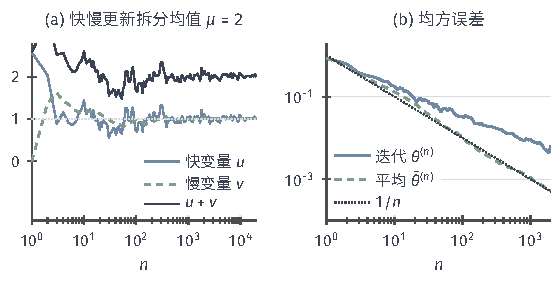
\includegraphics[width=94mm]{figures/03-optimization-evolution-and-signals/02-processes-and-trajectory-evolution/tikz/dtsp-fast-slow-averaging/figure.pdf}
  \caption{快慢更新与迭代平均（固定随机种子，横轴对数刻度）。(a)例~\ref{ex:dtsp-two-timescale}的一次运行，$Y$独立服从$\mathcal N(2,1)$，$\beta_n=(n+1)^{-0.6}$，$\alpha_n=(n+1)^{-0.9}$；点线为极限$1$。(b)均值递推$\theta^{(n+1)}=\theta^{(n)}+(n+1)^{-0.6}(Y_{n+1}-\theta^{(n)})$（$Y$独立服从$\mathcal N(1,1)$，$\theta^{(0)}=0$）的迭代与其累计平均在$200$次重复上的均方误差，点线为$1/n$。}
  \label{fig:dtsp-fast-slow-averaging}
\end{figure}

把这一观察推广为一般结论，需要在根附近对平均漂移作线性化（要求Jacobian的特征值实部为负）、噪声协方差收敛、步长满足$\frac12<\gamma<1$等条件，结论是平均迭代的缩放误差渐近正态，且协方差在一类估计中达到最小。这一结论关于估计效率与置信区间的统计含义属于统计推断部分；把递推在小步长下近似为随机微分方程的扩散逼近，留到第~\ref{chap:continuous-time-stochastic-processes}章，它们都不是本节主线结论的前提。
